\documentclass[10pt,twocolumn,letterpaper]{article}
\usepackage[review,datasets]{wacv}
\usepackage{amsmath,amssymb,booktabs,graphicx,microtype}
\definecolor{wacvblue}{rgb}{0.21,0.49,0.74}
\usepackage[pagebackref,breaklinks,colorlinks,allcolors=wacvblue]{hyperref}

\def\wacvPaperID{*****}
\def\confName{WACV}
\def\confYear{2027}

\title{Skin-Tone Steering at Matched Change:\\
A Preregistered Evaluation of Denoising-Time Latent Control in SDXL}
\author{Anonymous submission}
\date{}

\newcommand{\method}{stepwise latent steering}

\begin{document}
\maketitle

\begin{abstract}
We study whether a linear direction estimated from paired portrait latents can
control visible skin tone in Stable Diffusion XL while preserving other image
properties. The proposed method computes a paired mean difference in the VAE
latent space, applies a spatial Gaussian mask, and distributes the resulting
perturbation across denoising steps. We preregister a matched-change evaluation
after calibration, estimate the direction from 64 of 96 noise-coupled prompt
pairs, validate an image-colour instrument on the remaining 32, and evaluate
570 conditions over 30 held-out seeds. The parent study found no detectable
face-embedding advantage, but masking reduced LPIPS relative to unmasked
steering by 0.023 lighter and 0.082 darker (Holm-adjusted $p=.012,.002$).
We then prospectively fixed an independent-seed replication with new direction
data and 30 new seeds. Its LPIPS advantages were again positive: 0.024
($[0.005,0.041]$) lighter and 0.041 ($[0.018,0.065]$) darker. The locked
decision was nevertheless inconclusive: only 8 and 10 shared matched seeds
were available, below the minimum of 12, and the lighter two-test Holm value
was .056 (darker .019). The cross-campaign masked-direction cosine was 0.919.
The evidence supports a localized perceptual-preservation signal under this
SDXL protocol, not strict replication, identity preservation, disentanglement,
or bias mitigation. Skin tone is treated only as an apparent visual attribute,
never as a proxy for race or ethnicity.
\end{abstract}

\section{Introduction}

Latent diffusion models synthesize high-resolution images by denoising in a
compressed representation rather than directly in pixel space
\cite{rombach2022ldm}. SDXL extends this family with a larger U-Net and richer
conditioning \cite{podell2023sdxl}. These models offer expressive control but
also make it difficult to isolate one visual attribute without changing
identity, pose, or composition.

Linear semantic directions have been effective in GAN latent spaces
\cite{shen2020interfacegan}. We ask whether an analogous direction, estimated
from paired SDXL VAE encodings, can be used during diffusion sampling. Our
technical hypothesis is that a denoiser can absorb small perturbations injected
throughout sampling more coherently than a single post-hoc edit. Our scientific
hypothesis is narrower: at a matched change in measured skin tone, stepwise
masked injection will preserve non-target properties better than relevant
baselines.

We make three contributions. First, we specify the paired estimator and
denoising-time intervention. Second, we provide a preregistered matched-change
comparison and a prospectively specified independent-seed replication that
separate target response from preservation. Third, we release an auditable
research artifact with immutable model and data hashes, measurement validation,
seed-level uncertainty, missingness, and failures.

\section{Related work}

This study does not claim that semantic directions in diffusion models are
new. Asyrp identifies a semantic representation space inside frozen diffusion
U-Nets and manipulates directions across the reverse process
\cite{kwon2023asyrp}; later work discovers concept-specific internal directions
for text-to-image generation \cite{li2024directions}. Concept Sliders instead
learn low-rank parameter directions for continuous, composable control
\cite{gandikota2024sliders}. Our narrower object of study is a direction formed
directly from paired SDXL VAE encodings, added to scheduler latents throughout
sampling without optimization. The empirical question is whether that simple
intervention offers a preservation advantage at matched target response, not
whether diffusion representations admit semantic control in general.

\section{Construct and scope}

Race and ethnicity are social identities, not one-dimensional visual
attributes. The intervention in this study is therefore called a
\emph{skin-tone direction}. It must not be interpreted as changing, estimating,
or classifying race. Even datasets designed to balance face categories expose
the difficulty and consequences of reducing social categories to visual labels
\cite{karkkainen2021fairface}. The present method is intended for controlled
generative-model research and auditing, not profiling or decisions about
people.

\section{Method}

Let $E(x)$ be the deterministic posterior-mode encoding of an image under the
SDXL VAE. Given $n$ noise-coupled prompt pairs $(x_i^{L},x_i^{D})$ generated
with the same seed and prompt template but different skin-tone descriptors, the
raw direction is
\begin{equation}
  v = \frac{1}{n}\sum_{i=1}^{n}\left[E(x_i^{D})-E(x_i^{L})\right].
\end{equation}
Seed reuse controls the initial diffusion noise but does not guarantee the same
apparent identity after conditioning changes. Identity, composition, prompt
wording, and illumination therefore remain potential training-direction
confounders.

We multiply $v$ by a spatial mask $M\in[0,1]^{H\times W}$ centered on the face:
\begin{equation}
  M(p)=w_e+(w_c-w_e)\exp\left[-3\left(\frac{\lVert p\rVert_2}{r}\right)^2\right],
  \quad \tilde v=M\odot v,
\end{equation}
where the study uses center weight $w_c=1$, edge weight $w_e=0.3$, and radius
$r=1$. For $T$ reverse-diffusion steps and steering magnitude $\alpha$, the
pipeline updates the scheduler latent after each step by
\begin{equation}
  z_t \leftarrow z_t + \frac{\alpha}{T}\tilde v.
\end{equation}
The implementation uses 25 DPM-Solver++ multistep updates, motivated by fast
diffusion ODE solvers \cite{lu2022dpmsolver}, with classifier-free guidance 7.5.

\section{Evaluation design}

The target response and preservation outcomes must be measured separately.
The continuous target proxy uses cheek-pixel CIE Lab individual typology angle
(ITA). Instrumental ITA decreases as measured pigmentation increases
\cite{wilkes2015ita}, but apparent skin color in images is affected by hue,
illumination, and acquisition conditions and is not fully represented by a
single light--dark axis \cite{thong2023skin}. We therefore validate ordering and
prespecified illumination perturbations on a held-out split and describe the
result only as apparent image color.

The primary preservation outcome is face-embedding similarity, following the general
embedding approach of FaceNet \cite{schroff2015facenet}, at a matched continuous
skin-tone change. Secondary outcomes are LPIPS perceptual distance
\cite{zhang2018lpips}, background-only SSIM \cite{wang2004ssim}, head-pose
drift, face-detection failure, and monotonicity.

The confirmatory design used held-out seeds and four methods: prompt-only
generation, post-hoc latent addition, unmasked stepwise injection, and masked
stepwise injection. The preregistered configuration contains 30 held-out
generation seeds and method-specific grids frozen after calibration.
Comparisons are paired within seed. We report means, standard deviations,
medians, detector failures, and 95\% seed-level
bootstrap confidence intervals; secondary confirmatory tests use Holm
correction. A run cannot pass when a required metric is missing.

After fixing the parent result, we prospectively specified an independent-seed
replication with a newly generated 96-pair campaign, 64 pairs for a new
direction, 32 for the unchanged validation gates, and evaluation seeds
600000--600029. The model revision, method grids, target, tolerance, outcomes,
and bootstrap procedure remained fixed. The locked replication family contains
only the lighter- and darker-direction masked-versus-unmasked LPIPS contrasts.
Strict replication requires both positive estimates, both ordinary 95\%
bootstrap intervals above zero, and both two-test Holm-adjusted $p<.05$; either
nonpositive estimate is failure, while fewer than 12 shared matched seeds in
either direction is inconclusive. Parent and replication samples are reported
separately rather than pooled as a 60-seed confirmatory study.

\section{Pre-confirmatory validation and calibration}

The direction-data campaign generated 96 noise-coupled light/dark prompt pairs.
We reserve 64 pairs for direction estimation and 32 pairs for measurement
validation. The ITA instrument detected the face and cheek regions in all 32
held-out pairs, ordered the light-descriptor image above the dark-descriptor
image in 31 of 32 pairs (96.9\%), and produced a median within-pair separation
of 16.67 ITA degrees. Across prespecified brightness and white-balance
perturbations, the median absolute ITA shift was 0.40 degrees and the 95th
percentile was 3.06 degrees. Table~\ref{tab:validation} shows that every frozen
gate passed before confirmatory generation.

\begin{table}[t]
\centering
\caption{Held-out validation of the continuous image-colour instrument.}
\label{tab:validation}
\begin{tabular}{@{}lrr@{}}
\toprule
Criterion & Required & Observed \\
\midrule
Detection rate & $\geq 0.95$ & 1.000 \\
Pair-order accuracy & $\geq 0.90$ & 0.969 \\
Median pair gap (ITA) & $\geq 8.0$ & 16.67 \\
Median perturbation shift & $\leq 2.0$ & 0.40 \\
95th-percentile shift & $\leq 5.0$ & 3.06 \\
\bottomrule
\end{tabular}
\end{table}

Calibration used seeds disjoint from both the direction-data and confirmatory
sets. The frozen target was an absolute five-degree ITA change with a
three-degree matching tolerance. Prompt-only, unmasked stepwise, and masked
stepwise steering achieved both directions for all three calibration seeds.
Post-hoc addition achieved the darker target for all three seeds but the
lighter target for only one; wider endpoint probes remained non-monotonic and
identity-dependent. We therefore froze post-hoc addition as a descriptive
feasibility and dose-response baseline, excluding it from the primary matched
contrast before confirmatory generation.

\section{Confirmatory results}

\subsection{Completion and target response}

The runner produced all 570 prespecified condition rows with 570 unique keys
and the frozen configuration fingerprint. All images generated. One post-hoc
condition (seed 500019, $\alpha=-1.5$) lacked a detectable edited face/skin
region, leaving 569 metric-complete rows (99.8\%). The failure remains in the
missingness denominator. All 330 conditions in the primary matched-change
methods were complete.

Figure~\ref{fig:dose} shows the mean target response. Mean seed-level Spearman
correlations between $\alpha$ and skin-tone change were 0.95 for prompt-only,
0.93 for unmasked stepwise, 0.92 for masked stepwise, and 0.67 for post-hoc
addition. The post-hoc median was 0.99 but its mean 95\% interval was
$[0.43,0.88]$, confirming substantial seed dependence.

\begin{figure*}[t]
  \centering
  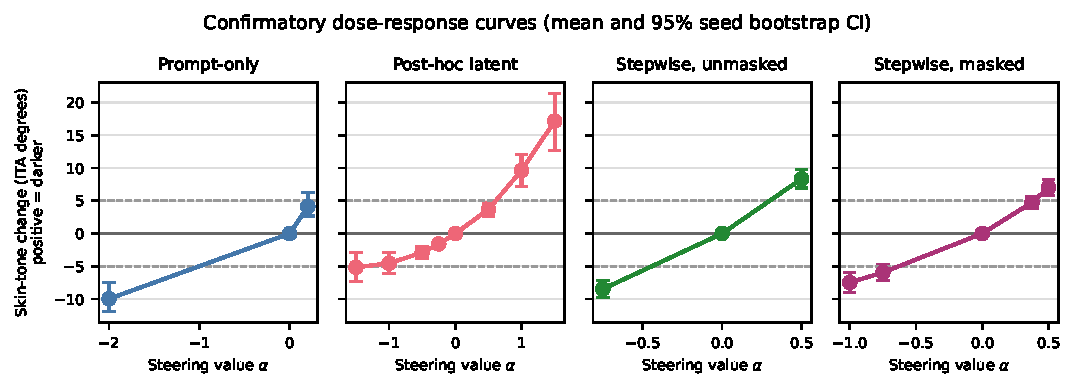
\includegraphics[width=\textwidth]{../figures/confirmatory_dose_response.pdf}
  \caption{Confirmatory dose-response curves. Points are seed means and bars
  are 95\% seed-level bootstrap intervals. Dashed lines mark the prespecified
  $\pm5$ ITA targets; positive change denotes a darker measured appearance.}
  \label{fig:dose}
\end{figure*}

The target was reached within the three-degree tolerance unevenly
(Table~\ref{tab:coverage}). Masked steering had the highest coverage in both
directions. Among successful matches, its mean achieved changes were 5.06 ITA
lighter and 5.23 ITA darker. Low prompt-only lighter coverage constrains that
stratum to six seeds shared with the masked reference.

\begin{table}[t]
\centering
\caption{Prespecified matched-target coverage over 30 seeds.}
\label{tab:coverage}
\begin{tabular}{@{}lrr@{}}
\toprule
Method & Lighter & Darker \\
\midrule
Prompt-only & 7 (23\%) & 18 (60\%) \\
Stepwise, unmasked & 13 (43\%) & 15 (50\%) \\
Stepwise, masked & 19 (63\%) & 26 (87\%) \\
\bottomrule
\end{tabular}
\end{table}

\subsection{Preservation at matched change}

The primary face-similarity hypothesis was not supported. Masked-stepwise
advantages relative to prompt-only were $-0.0008$ (95\% CI
$[-0.0035,0.0016]$, $n=6$) for lighter edits and 0.0032
($[-0.0056,0.0149]$, $n=17$) for darker edits. Relative to unmasked
stepwise steering, the advantages were 0.0020 ($[-0.0014,0.0056]$, $n=13$)
and 0.0079 ($[-0.0027,0.0184]$, $n=14$). All Holm-adjusted $p$ values were
1.0.

Masking nevertheless improved perceptual preservation relative to unmasked
steering: the paired LPIPS advantage was 0.0235 ($[0.0128,0.0360]$,
$p_{\mathrm{Holm}}=.012$) for lighter edits and 0.0825
($[0.0476,0.1302]$, $p_{\mathrm{Holm}}=.002$) for darker edits. Against
prompt-only generation, the darker-direction LPIPS advantage was 0.0812
($[0.0379,0.1218]$, $p_{\mathrm{Holm}}=.028$). The corresponding
darker-direction improvements were 0.0207 in background SSIM
($[0.0105,0.0319]$, $p_{\mathrm{Holm}}<.001$) and 1.61 in the pose-difference
proxy ($[0.88,2.36]$, $p_{\mathrm{Holm}}=.007$). Masking also improved
background SSIM by 0.0129 versus unmasked darker edits
($[0.0080,0.0176]$, $p_{\mathrm{Holm}}=.002$). No other secondary contrast
survived Holm correction. Figure~\ref{fig:contrasts} shows every prespecified
matched preservation contrast, including null and adverse estimates.

\begin{figure*}[t]
  \centering
  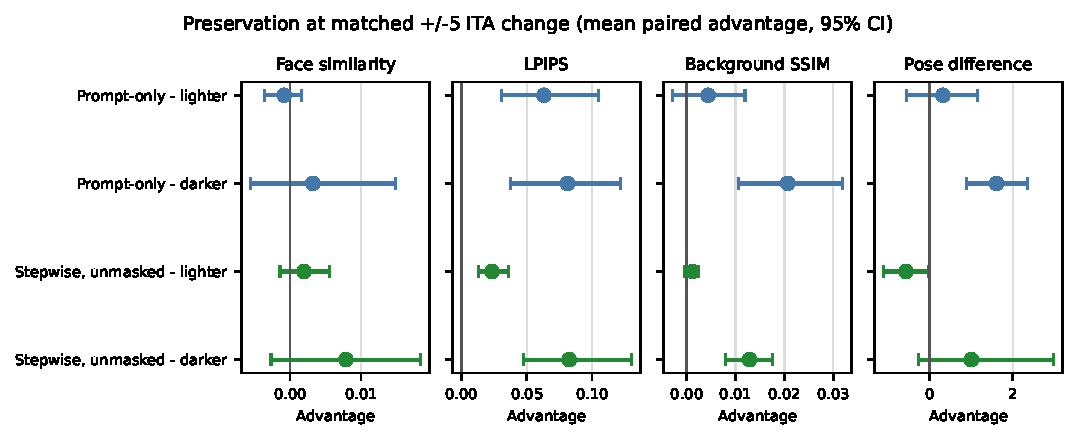
\includegraphics[width=\textwidth]{../figures/confirmatory_matched_contrasts.pdf}
  \caption{Masked-stepwise preservation advantage at matched $\pm5$ ITA
  change. Bars are 95\% seed-level bootstrap intervals. Positive values favor
  masked steering after orienting every outcome so that larger is better.}
  \label{fig:contrasts}
\end{figure*}

Figure~\ref{fig:qualitative} is illustrative rather than inferential. Its seed
was selected by a fixed rule: maximize the number of complete matched rows,
then choose the seed closest to the median base ITA, breaking ties by lower
seed. The prompt-only example visibly demonstrates why matched image-colour
change does not imply matched identity or composition.

\begin{figure*}[t]
  \centering
  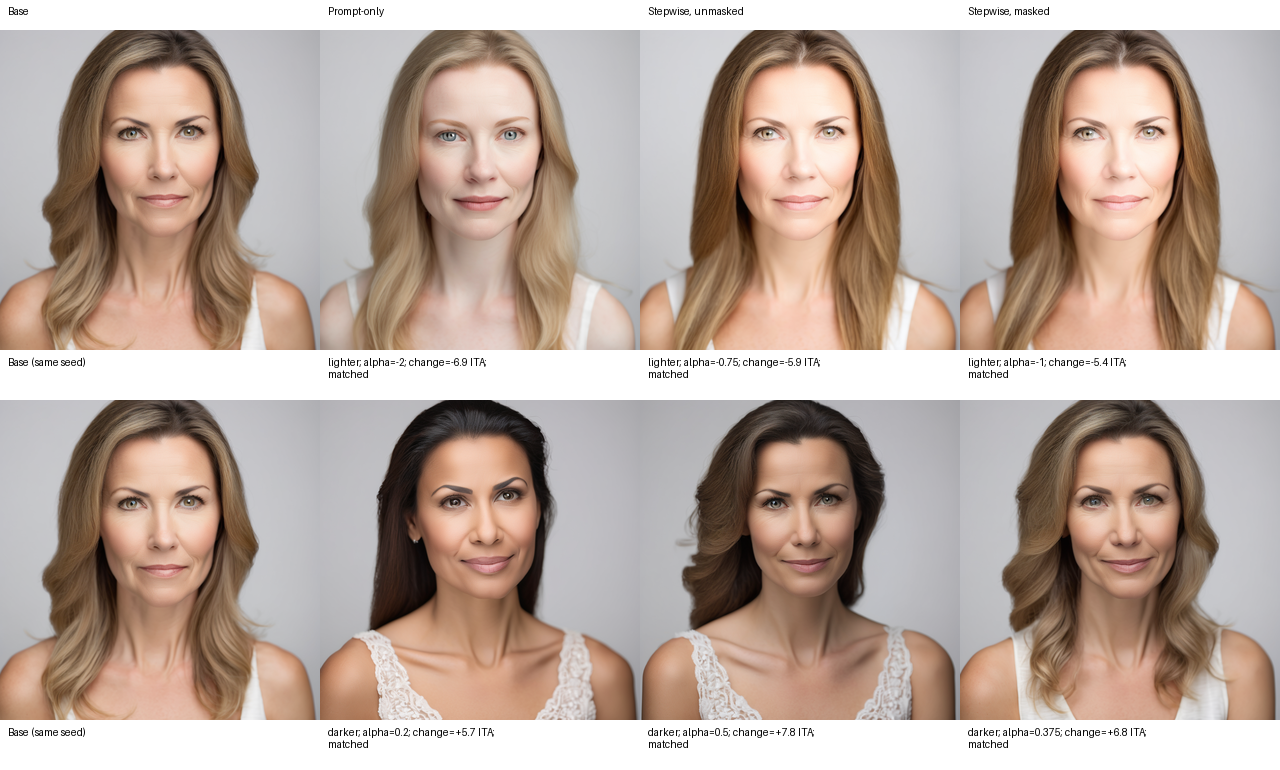
\includegraphics[width=\textwidth]{../figures/confirmatory_qualitative.png}
  \caption{Deterministically selected confirmatory example (seed 500011).
  Each row reuses the same base image; labels report the selected alpha and
  achieved ITA change. Prompt-only conditioning can alter apparent identity
  despite reusing the diffusion seed.}
  \label{fig:qualitative}
\end{figure*}

\section{Post-confirmatory robustness}

We performed two explicitly exploratory checks after completing the frozen
analysis. First, we repeated matching with one- and two-degree ITA tolerances.
The LPIPS advantage retained the same positive direction in every estimable
stratum, and face-similarity estimates remained compatible with no advantage.
However, shared matched samples collapsed to $n=1$--5 at one degree and
$n=3$--12 at two degrees; no secondary contrast survived Holm correction.
Thus, the preregistered three-degree results should not be interpreted as
evidence of precisely matched effects under stricter tolerances.

Second, we re-encoded all 64 training pairs and confirmed that the resulting
direction was exactly equal to the recorded confirmatory tensor (maximum
absolute difference zero). We then drew 200 random disjoint split-halves at
each pair count. Table~\ref{tab:stability} reports cosine agreement between
independently estimated directions. Stability increased with sample size, and
masking improved agreement, but even two disjoint 32-pair estimates had median
cosine 0.75 before masking and 0.82 after masking. The direction is therefore
reproducible under the fixed 64-pair campaign but not sample-invariant.

\begin{table}[t]
\centering
\caption{Exploratory split-half direction stability. Entries are median cosine
similarity with 2.5th--97.5th percentiles over 200 disjoint resamples.}
\label{tab:stability}
\begin{tabular}{@{}rrr@{}}
\toprule
Pairs/half & Raw direction & Masked direction \\
\midrule
8  & 0.42 [0.28, 0.53] & 0.53 [0.38, 0.63] \\
16 & 0.59 [0.50, 0.66] & 0.69 [0.60, 0.75] \\
32 & 0.75 [0.69, 0.78] & 0.82 [0.77, 0.84] \\
\bottomrule
\end{tabular}
\end{table}

\section{Prospective independent-seed replication}

A fresh 96-pair campaign passed the unchanged held-out measurement gates before
outcome generation: detection was 1.000, pair ordering 0.969, the median pair
gap 16.08 ITA degrees, and median/95th-percentile perturbation shifts 0.35/3.83
degrees. The new outcome run then completed all 570 frozen conditions over 30
new seeds. All images generated; one post-hoc condition (seed 600020,
$\alpha=-1.5$) retained a face/skin-region measurement failure, leaving 569
metric-complete rows and every primary matched method complete.

Masked target coverage was 18/30 lighter and 27/30 darker, versus 10/30 in each
direction for unmasked steering and 7/30 lighter and 22/30 darker for
prompt-only. The locked masked-versus-unmasked LPIPS effects retained the
parent signs and had ordinary bootstrap intervals above zero
(Table~\ref{tab:replication}). The formal decision was nevertheless
\emph{inconclusive coverage}: only 8 lighter and 10 darker seeds were shared
between matched methods, below the prespecified minimum of 12. Even without
that override, the lighter two-test Holm value of .056 missed the strict rule;
the darker value was .019. We therefore report a sign-consistent,
interval-positive pattern, not strict or directional replication.

\begin{table}[t]
\centering
\caption{Locked independent-seed replication family. Advantage is unmasked
LPIPS minus masked LPIPS; positive values favor masking. $p_{H(2)}$ is Holm
adjusted across these two tests.}
\label{tab:replication}
\begin{tabular}{@{}lrrrr@{}}
\toprule
Direction & $n$ & Advantage & 95\% CI & $p_{H(2)}$ \\
\midrule
Lighter & 8  & 0.0238 & [0.0049, 0.0415] & .0555 \\
Darker  & 10 & 0.0409 & [0.0176, 0.0655] & .0192 \\
\bottomrule
\end{tabular}
\end{table}

The independently estimated raw directions had cosine 0.884; applying the
frozen spatial mask raised cross-campaign cosine to 0.919. Their norm ratio was
1.04. Figure~\ref{fig:replication} compares effects and target coverage without
pooling the two campaigns.

\begin{figure*}[t]
  \centering
  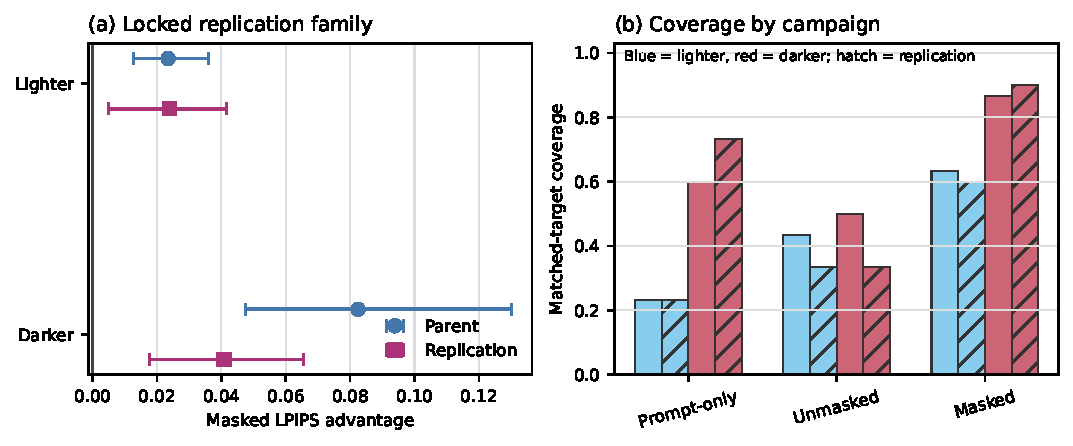
\includegraphics[width=\textwidth]{../figures/replication_comparison.pdf}
  \caption{Parent and prospective replication reported separately. (a) Locked
  masked-versus-unmasked LPIPS advantages with ordinary 95\% bootstrap
  intervals. (b) Matched-target coverage; hatching marks replication bars.
  The formal replication decision is inconclusive because shared matched
  coverage fell below 12 in both directions.}
  \label{fig:replication}
\end{figure*}

\section{Limitations}

The study evaluates one generator, scheduler, resolution, and model revision;
cross-model generalization is unknown. Synthetic direction pairs can encode
prompt wording, brightness, age, gender presentation, hair, or facial features
alongside skin tone, and seed reuse does not preserve identity. A center
Gaussian is not a semantic skin mask. The same generator creates direction and
evaluation images, so model-specific artifacts may dominate. ITA is an
image-colour proxy, not a complete representation of skin appearance, and its
validation uses synthetic prompt pairs rather than calibrated physical colour
measurements. Face embeddings and face/skin detectors can exhibit demographic
error. Matched-change coverage is incomplete and particularly low for
prompt-only lighter edits, reducing paired sample sizes and precision. The
post-confirmatory tolerance analysis confirms that stricter matching is too
sparse for stable inference, while the split-half analysis shows that the
learned direction remains sensitive to which synthetic pairs are sampled. The
prospective replication independently reproduced the effect signs and
direction geometry but remained formally inconclusive because shared matched
coverage was only 8--10 seeds. Both campaigns use the same generator, prompt
template, descriptors, and calibration grids, so this is seed-level rather
than model- or construct-level independence. The
closest-grid matching rule also selects on a noisy measured response; denser
grids or prespecified dose--response interpolation would reduce that source of
selection and residual mismatch. The
pose measure is a five-landmark proxy rather than a full 3D estimator. No human
study assesses perceived identity, realism, or social harms. Finally, the
additive update is scheduler-dependent and has not been validated across model
or library revisions.

\section{Conclusion}

In the parent campaign, masked denoising-time injection offered higher target
coverage than the tested unmasked grid and improved LPIPS preservation in both
directions. A prospectively specified new-seed campaign produced smaller but
same-sign LPIPS advantages with intervals above zero and high cross-campaign
direction cosine. Its locked decision was inconclusive because only 8--10
shared matched seeds were available, and the lighter multiplicity-adjusted
test narrowly missed .05. The preregistered face-similarity hypothesis was not
supported in either campaign's broader corrected family. The result must not
be described as strict replication, identity preservation, disentanglement,
or bias mitigation. The principal contribution is a bounded empirical signal
and an auditable protocol for separating target response, preservation,
missingness, and unsupported social claims.

{\small
\bibliographystyle{ieeenat_fullname}
\bibliography{../references}
}
\end{document}
